\section{M-step}

The article miss at providing a full understanding on how Radial basis functions are used to compute exactly the M-step. In order to implement safely, it is of interest to write down all the analytic computations. So let's start from the beginning:\\

At iteration $k$, in the M-step, we assume that the state sequence $(x_t)_{t=1 \ldots T}$ follow the probability $q \left(x_1, \ldots ,x_T \right)$ such that the state $x_t$ follow the Gaussian probability:
\begin{align*}
  q(x_t) = \mathcal{N}\left( \hat{x}_{t \given T}, \hat{P}_{t \given T} \right), \  t=1 \ldots T\\
\end{align*}
and that the joint states $(x_t, x_{t+1})$ follow the Gaussian probability:
\begin{align*}
  q(x_t, x_{t+1}) &=
  \mathcal{N}
    \left(
      \left[
        \begin{array}{c} \hat{x}_{t \given T} \\ \hat{x}_{t+1 \given T} \end{array}
      \right],
      \left[
        \begin{array}{cc} \hat{P}_{t \given T} & \hat{P}_{t,t+1 \given T}\\ \hat{P}_{t,t+1 \given T} & \hat{P}_{t+1 \given T} \end{array}
      \right]
    \right), \  t=1 \ldots T-1\\
\end{align*}
where the quantities the means $\hat{x}_{t \given T}$ and covariance matrices $\hat{P}_{t \given T}, \hat{P}_{t,t+1 \given T}$ were computed in the E-step.
We adopt the following notations:
\begin{align*}
  q_t(x) &= q(x = x_t)\\
  q_{t,t+1}(x,x') &= q \left((x,x') = (x_t, x_{t+1})\right)\\
\end{align*}

Now we want to compute the updated parameter $\theta^{(k)} = \left( \theta_f^{(k)}, \theta_g^{(k)}, Q^{(k)}, R^{(k)} \right)$.

The updated parameter $\theta^{(k)}$ is the maximizer of the expected complete likelihood $L_q$ which is equal to the maximizer of the expected complete log-likelihood $l_q$:
\begin{align*}
  \theta^{(k)} &= \underset{\theta}{\text{argmax }}L_q(\theta) = \underset{\theta}{\text{argmax }}l_q(\theta)\\
\end{align*}
First we need to express $l_q(\theta)$ using the graph factorization.
Our graphical model is the following :
\begin{figure}[H]
	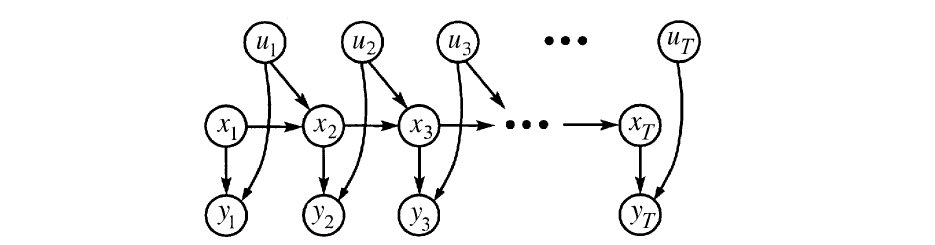
\includegraphics[width=14cm]{screenshot_graphical_model.PNG}
	\captionof{figure}{Graphical model of our system.}
\end{figure}
Firstly, the inputs $u_t$ are not modeled as random variable, so we won't take them into account in the factorization.
%\notes{If $u_t$ were random variables, we wouldn't have a tree anymore and the inference that we did in the E-Step would be complicated.}
Thus, the factorization over the graph yields :
\begin{align*}
p_{\theta}(x_1, \ldots x_T, y_1, \ldots , y_T) &= p_{\theta}(x_1) \prod_{t=1}^{T-1}{p_{\theta}(x_{t+1} \given x_t)} \prod_{t=1}^{T}{p_{\theta}(y_t \given x_t)}\\
\end{align*}
Thus, the likelihood of the observed the sequence $\overline{y} = (\overline{y}_t)_{t=1 \ldots T}$ is :
\begin{align*}
  p_{\theta}(x_1, \ldots x_T, \overline{y}_1, \ldots , \overline{y}_T) &= p_{\theta}(x_1) \prod_{t=1}^{T-1}{p_{\theta}(x_{t+1}\given x_t)} \prod_{t=1}^{T}{p_{\theta}(\overline{y}_t \given x_t)}\\
\end{align*}
Taking the $\log$ and expectation of this likelihood over the probability $q \left(x_1, \ldots ,x_T \right)$ gives us the expected log-likelihood:
\begin{align*}
  l_q(\theta) & =
    \mathbb{E}_q(\log(p_{\theta}(x_1))) +
    \sum_{t=1}^{T-1}{\mathbb{E}_q \left( \log(p_{\theta}(x_{t+1} \given x_t)) \right)} +
    \sum_{t=1}^{T}{\mathbb{E}_q\left( \log(p_{\theta}(\overline{y}_t \given x_t)) \right)}
  \\
  \mathbb{E}_q(\log(p_{\theta}(x_1))) &= -\frac{1}{2}\int_x{q_1(x) (x - \hat{x}_{1 \given 1})^{\top} \hat{P}_{1 \given 1}^{-1} (x - \hat{x}_{1 \given 1}) dx}
  \\
  \mathbb{E}_q \left( \log(p_{\theta}(x_{t+1} \given x_t)) \right) &= -\frac{1}{2}\int_{x,x'}{q_{t,t+1}(x, x') ((x' - f(x,u_t))^{\top} Q^{-1} (x' - f(x,u_t)) dxdx'}\\
  \mathbb{E}_q\left( \log(p_{\theta}(\overline{y}_t \given x_t)) \right) &= -\frac{1}{2}\int_x{q_t(x) (\overline{y}_t - g(x, u_t))^{\top} R^{-1} (\overline{y}_t - g(x, u_t)) dx}\\
\end{align*}
Firstly, to get rid of the multiplying constants $-\frac{1}{2}$, we multiply the expected log likelihood by $-2$ such that our maximization problem becomes a minimization problem :
\begin{align*}
  \theta^{(k)} &= \underset{\theta}{\text{argmin }}l(\theta)\\
\end{align*}
Then we notice that the expectation $\mathbb{E}_q(\log(p_{\theta}(x_1)))$ is constant with respect to $\theta$ so it doesn't account for the maximization.
Introducing the author notations :
\begin{align*}
  \Phi_f(x, u) &= [\rho_1(x), \ldots , \rho_I(x), x^{\top}, u^{\top}, 1]^{\top}\\
  \Phi_g(x, u) &= [\rho'_1(x), \ldots , \rho'_J(x), x^{\top}, u^{\top}, 1]^{\top}\\
  \left< F(.) \right>_{t} &= \int_x{q_t(x) F(x) dx} = \mathbb{E}_q \left( F(x_t) \right)\\
  \left< F(.) \right>_{t,t+1} &= \int_{x, x'}{q_{t,t+1}(x, x') F(x,x') dx}dx' = \mathbb{E}_q \left( F(x_t, x_{t+1}) \right)\\
\end{align*} % NOTA : on ne devrait pas avoir les mêmes x et u pour f et g
such that:
\begin{align*}
  f(x,u) = \theta_f \Phi_f(x, u)\\
  g(x,u) = \theta_g \Phi_g(x, u)\\
\end{align*}
and the functions $l^1_q$ and $l^2_q$:
\begin{align*}
  l^1_q(\theta_f, Q) &= \sum_{t=1}^{T-1}\left< (x, x') \mapsto (x' - \theta_f\Phi_f(x,u_t))^{\top} Q^{-1}(x' - \theta_f\Phi_f(x,u_t)) \right>_{t,t+1} + (T-1) \log( \given Q \given )
  \\
  l^2_q(\theta_g, R) &= \sum_{t=1}^{T}\left< x \mapsto (\overline{y}_{t} - \theta_g \Phi_g(x, u_t))^{\top} R^{-1} (\overline{y}_{t} - \theta_g \Phi_g(x, u_t)) \right>_{t} + T \log( \given R \given )
  \\
\end{align*}
our minimization problem becomes:
\begin{align*}
  \left(\theta_f^{(k)}, Q^{(k)}\right) &= \underset{\theta_k, Q}{\text{argmin }}l^1_q(\theta_f, Q)\\
  \left(\theta_g^{(k)}, R^{(k)}\right) &= \underset{\theta_g, R}{\text{argmin }}l^2_q(\theta_g, R)\\
\end{align*}
At the minimum point, the gradients vanish
\begin{align*}
  \left[
    \begin{array}{c} \nabla_{\theta_f} l^1_q \\ \nabla_{Q} l^1_q \end{array}
  \right] \left(\theta_f^{(k)}, Q^{(k)}\right) &=
  \left[
    \begin{array}{c} 0 \\ 0 \end{array}
  \right]\\
  \left[
    \begin{array}{c} \nabla_{\theta_g} l^2_q \\ \nabla_{R} l^2_q \end{array}
  \right] \left(\theta_g^{(k)}, R^{(k)} \right) &=
  \left[
    \begin{array}{c} 0 \\ 0 \end{array}
  \right] \\
\end{align*}
which yields:
\begin{align*}
  \theta_f^{(k)} &=
    \left(
      \sum_{t=1}^{T-1}{\left< x' \mapsto x' \Phi_f(x,u_t)^{\top} \right>_{t+1}}
    \right)
    \left(
      \sum_{t=1}^{T-1}{\left< x \mapsto \Phi_f(x, u_t)\Phi_f(x,u_t)^{\top} \right>_{t}}
    \right)^{-1}
  \\
  Q^{(k)} &=
    \frac{1}{T-1}
    \left(
      \sum_{t=1}^{T-1}{\left< x' \mapsto x'x'^{\top} \right>_{t+1}} -
      \theta_f^{(k)} \sum_{t=1}^{T-1}{\left< (x,x') \mapsto \Phi_f(x, u_t) x'^{\top} \right>_{t,t+1}}
    \right)
  \\
  \theta_g^{(k)} &=
    \left(
      \sum_{t=1}^{T}{\left< x \mapsto \overline{y}_{t}\Phi_g(x,u_t)^{\top} \right>_{t}}
    \right)
    \left(
      \sum_{t=1}^{T}{\left< x \mapsto \Phi_g(x,u_t)\Phi_g(x,u_t)^{\top} \right>_{t}}
    \right)^{-1}
  \\
  R^{(k)} &=
    \frac{1}{T}
    \left(
      \sum_{t=1}^{T}{\overline{y}_t \overline{y}_t^{\top}} -
      \theta_g^{(k)} \sum_{t=1}^{T}{\left< x \mapsto \Phi_f(x, u_t) \overline{y}_t^{\top} \right>_{t}}
    \right)
  \\
\end{align*}
Now the keypoint is to compute these expectations.
To compute $\theta_f^{(k)}$ and $Q^{(k)}$, we need to compute the expectations:
\begin{align*}
  \left< (x,x') \mapsto x' \Phi_f(x,u_t)^{\top} \right>_{t,t+1} &=
    \left< (x,x') \mapsto [x'\rho_1(x), \ldots , x'\rho_I(x), x'x^{\top}, x'u^{\top}, x']\right>_{t,t+1}
  \\
  \left< (x,x') \mapsto \Phi_f(x, u_t) x'^{\top} \right>_{t,t+1} &=
    \left< (x,x') \mapsto [x'\rho_1(x), \ldots , x'\rho_I(x), x'x^{\top}, x'u^{\top}, x']^{\top} \right>_{t,t+1}
  \\
  \left< x \mapsto \Phi_f(x, u_t)\Phi_f(x,u_t)^{\top} \right>_{t} &=
    \left< x \mapsto \left[
      \begin{array}{cccccc}
        \rho_1(x)\rho_1(x) & \ldots & \rho_1(x)\rho_I(x) & \rho_1(x)x^{\top} & \rho_1(x)u^{\top} & \rho_1(x) \\
        \ldots & \ldots & \ldots & \ldots & \ldots & \ldots\\
        \rho_I(x)\rho_1(x) & \ldots & \rho_I(x)\rho_I(x) & \rho_I(x)x^{\top} & \rho_I(x)u^{\top} & \rho_I(x) \\
        \rho_I(x)x & \ldots & \rho_I(x)x & xx^{\top} & xu^{\top} & x \\
        \rho_I(x)u & \ldots & \rho_I(x)u & xu^{\top} & uu^{\top} & u \\
        \rho_I(x) & \ldots & \rho_I(x) & x^{\top} & u^{\top} & 1 \\
      \end{array}
    \right]
  \right>_{t}
  \\
  \left< x' \mapsto x'x'^{\top} \right>_{t+1} &\\
\end{align*}
So we need to compute the elementary expectations:
\begin{align*}
  &\left< (x,x') \mapsto \rho_i(x) x' \right>_{t,t+1}\\
  &\left< (x,x') \mapsto x'x^{\top} \right>_{t,t+1}\\
  &\left< (x,x') \mapsto x' \right>_{t,t+1}\\
  &\left< x' \mapsto x'x'^{\top} \right>_{t+1}\\
  &\left< x \mapsto \rho_i(x)\rho_j(x) \right>_{t}\\
  &\left< x \mapsto \rho_i(x) x \right>_{t}\\
  &\left< x \mapsto \rho_i(x) \right>_{t}\\
  &\left< x \mapsto xx^{\top} \right>_{t}\\
  &\left< x \mapsto x \right>_{t}\\
\end{align*}
We begin with the simple ones :
\begin{align*}
  \left< x' \mapsto x'\right>_{t+1} &= \hat{x}_{t+1 \given T}\\
  \left< (x,x') \mapsto x'x^{\top}\right>_{t,t+1} &= \hat{x}_{t+1 \given T} \hat{x}_{t \given T}^{\top} + \hat{P}_{t,t+1 \given T}\\
  \left< x \mapsto xx^{\top}\right>_{t} &= \hat{x}_{t \given T} \hat{x}_{t \given T}^{\top} + \hat{P}_{t \given T}\\
  \left< x \mapsto x\right>_{t} &= \hat{x}_{t \given T}\\
\end{align*}
For the other expectations, the authors make us observe that when we multiply the RBF function $\rho_i$ and $q_t$, we obtain a Gaussian density in $\mathbb{R}^p$ with mean $\mu^i_t$ and covariance $\Sigma^i_t$ :
\begin{align*}
  \Sigma^i_t &= \left( \hat{P}_{t \given T}^{-1} + S_i^{-1} \right)^{-1}\\
  \mu^i_t &= \Sigma^i_t \left( \hat{P}_{t \given T}^{-1} \hat{x}_{t \given T} + S_i^{-1}c_i \right)\\
\end{align*}
multiplied by the constant $\beta^i_t$ (due to non-normalization):
\begin{align*}
  \beta^i_t &= (2\pi)^{-p/2} |S_i|^{-1/2} |\hat{P}_{t|T}|^{-1/2} |\Sigma^i_t|^{1/2} \exp(-\frac{1}{2} \delta^i_t)\\
  \delta^i_t &= c_i^{\top} S_i^{-1} c_i + \hat{x}_{t \given T}^{\top} \hat{P}_{t \given T}^{-1} \hat{x}_{t \given T} - {\mu^i_t}^{\top} \Sigma^i_t \mu^i_t\\
\end{align*}
Using these notations, the expectations involving $x_t$ and $\rho_i$ can be computed:
\begin{align*}
  \left< x \mapsto \rho_i(x) x \right>_{t} &= \beta^i_t \mu^i_t\\
  \left< x \mapsto \rho_i(x) \right>_{t} &= \beta^i_t\\
\end{align*}
Identically, when we multiply the product $\rho_i \rho_j$ and $q_t$, we obtain a Gaussian density in $\mathbb{R}^p$ with mean $\mu^{i,j}_t$ and covariance $\Sigma^{i,j}_t$ :
\begin{align*}
  \Sigma^{i,j}_t &= \left( \hat{P}_{t \given T}^{-1} + S_i^{-1} + S_j^{-1} \right)^{-1}\\
  \mu^{i,j}_t &= \Sigma^{i,j}_t \left( \hat{P}_{t \given T}^{-1} \hat{x}_{t \given T} + S_i^{-1}c_i + S_j^{-1}c_j \right)\\
\end{align*}
multiplied by the constant $\beta^{i,j}_t$ (due to non-normalization):
\begin{align*}
  \beta^{i,j}_t &= (2\pi)^{-p} |S_i|^{-1/2} |S_j|^{-1/2} |\hat{P}_{t|T}|^{-1/2} |\Sigma^{i,j}_t|^{1/2} \exp(-\frac{1}{2} \delta^{i,j}_t)\\
  \delta^{i,j}_t &= c_i^{\top} S_i^{-1} c_i + c_j^{\top} S_j^{-1} c_j + \hat{x}_{t \given T}^{\top} \hat{P}_{t \given T}^{-1} \hat{x}_{t \given T} - {\mu^{i,j}_t}^{\top} {\Sigma^{i,j}_t}^{-1} \mu^{i,j}_t\\
\end{align*}
and the expectation involving the product $\rho_i \rho_j$ is:
\begin{align*}
  \left< x \mapsto \rho_i(x)\rho_j(x)\right>_{t} &= \beta^{i,j}_t\\
\end{align*}
Finally, when we multiply the RBF function $\rho_i$ and $q_{t,t+1}$, we obtain a Gaussian density in $\mathbb{R}^{2p}$ with mean $\mu^i_{t,t+1}$ and covariance $\Sigma^i_{t,t+1}$ :
\begin{align*}
  \Sigma^i_{t,t+1} &=
    \left(
      \left[
        \begin{array}{cc} \hat{P}_{t \given T} & \hat{P}_{t,t+1 \given T}\\ \hat{P}_{t,t+1 \given T} & \hat{P}_{t+1 \given T} \end{array}
      \right]^{-1}
       +
      \left[
        \begin{array}{cc} S_i^{-1} & 0\\ 0 & 0 \end{array}
      \right]
    \right)^{-1}
  \\
  \mu^i_{t,t+1} &= \Sigma^i_{t,t+1}
    \left(
      \left[
        \begin{array}{cc} \hat{P}_{t \given T} & \hat{P}_{t,t+1 \given T}\\ \hat{P}_{t,t+1 \given T} & \hat{P}_{t+1 \given T} \end{array}
      \right]^{-1}
      \left[
        \begin{array}{c} \hat{x}_{t \given T} \\ \hat{x}_{t+1 \given T} \end{array}
      \right] +
      \left[
        \begin{array}{c} S_i^{-1}c_i \\ 0 \end{array}
      \right]
    \right)
  \\
\end{align*}
multiplied by a constant $\beta^{i}_{t,t+1}$ :
\begin{align*}
  \beta^i_{t,t+1} &= (2\pi)^{-p/2} |S_i|^{-1/2} |\hat{P}_{t|T}|^{-1/2} |\Sigma^i_{t,t+1}|^{1/2} \exp(-\frac{1}{2} \delta^i_{t,t+1})\\
  \delta^i_{t,t+1} &= c_i^{\top} S_i^{-1} c_i + \hat{x}_{t \given T}^{\top} \hat{P}_{t \given T}^{-1} \hat{x}_{t \given T} - {\mu^i_{t,t+1}}^{\top} {\Sigma^i_{t,t+1}}^{-1} \mu^i_{t,t+1}\\
\end{align*}
Thus the last expectation is :
\begin{align*}
  \left< (x,x') \mapsto \rho_i(x) x' \right>_{x_{t}, x_{t+1}} &= \beta^i_{t,t+1}\\
\end{align*}

The interest of the RBF functions is that the expectations can be computed analytically and efficiently.
Otherwise, as soon as the state space dimension is big (for example $\geq 5$), these expectations must be estimmated, which is very expensive.
